\documentclass{beamer} %[compress, blue]
\mode<presentation>

\setbeamercolor{frametitle}{fg=lightred,bg=darkred}
\setbeamercolor{title}{fg=lightred,bg=darkred}
\usepackage[spanish,english]{babel}
\usepackage{ucs}
\usepackage{times}
\usepackage[T1]{fontenc}
\usepackage{tipa} %ŋ character
\usepackage[utf8x]{inputenc}
\usepackage[absolute,overlay]{textpos}
\usepackage{graphicx}
%\usepackage[small,bf]{caption}
%\usepackage{tabularx}
\usepackage{tikz}
\usepackage{url}
\usepackage{gb4e}
\usepackage{linguex}
\usepackage{cgloss4e}
\usepackage{multirow}
\usepackage{ragged2e} 
\usepackage{wasysym}
\usepackage{alltt}

\usetheme{Warsaw}

\definecolor{darkred}{RGB}{153,0,0}
\definecolor{lightred}{RGB}{226,200,200}
\definecolor{ranis}{RGB}{ 128,128,128}

\newcommand\cyrtext[1]{{\fontencoding{T2A}\selectfont #1}}
\newcommand\grktext[1]{{\fontencoding{LGR}\fontfamily{pmt}\selectfont #1}}

\useoutertheme[subsection=false]{smoothbars}

%\usecolortheme{seahorse} %beetle, albatross, fly, default light, seahorse, crane, dove
\usecolortheme[named= darkred]{structure}

\setbeamertemplate{footline}[text line]{} % makes the footer EMPTY
\setbeamertemplate{headline}[text line]{} % header empty

\setbeamersize{text margin left=0.5cm}
\setbeamertemplate{navigation symbols}{}


%\logo{
\includegraphics[height=1.6cm]{logoLAW.png}}
\pgfdeclareimage[height=1.6cm]{logo}{logoLAWnotrans.png}

\setlength{\TPHorizModule}{1mm}
\setlength{\TPVertModule}{1mm}

\newcommand{\MyLogoCentred}{
\begin{textblock}{14}(57.2,10.5)
  \pgfuseimage{logo}
\end{textblock}
}

\newcommand{\MyLogoBottomCentred}{
\begin{textblock}{14}(53.5,70)
  \pgfuseimage{logo}
\end{textblock}
}

\newcommand{\MyLogoBottomRight}{
\begin{textblock}{14}(112.2,80.0)
  \pgfuseimage{logo}
\end{textblock}
}

\newcommand{\MyLogo}{
\begin{textblock}{14}(112.2,0.5)
  \pgfuseimage{logo}
\end{textblock}
}

\date{3rd May 2011}
\title{Session 3: Morphological disambiguation}

\author{Felipe Sánchez-Martínez}

\begin{document}


\frame{\titlepage \MyLogoBottomCentred}


\begin{frame}
  \frametitle{Morphological disambiguation: table of contents}
  \tableofcontents
\end{frame}


\section{Lexical ambiguity and part-of-speech tagging}

\begin{frame}
  \frametitle{Lexical ambiguity and part-of-speech tagging /1}

  \begin{block}{Lexical ambiguity}
    A surface form with more than one possible morphological analysis\\
    Ex. \texttt{[en]} \emph{book} (\texttt{noun} or \texttt{verb})\\
    ~~$\rightarrow$ \texttt{[fr]} \emph{livre} (\texttt{noun})\\
    ~~$\rightarrow$ \texttt{[fr]} \emph{réserver} (\texttt{verb})\\
  \end{block}

  \begin{alertblock}{Do not confuse with polysemy!}
    A lemma and part-of-speech tag that have several meanings\\ %which may be
    %translated differently into the target language\\
    Ex. \texttt{[en]} \emph{bank} (\texttt{noun}) \\
    ~~$\rightarrow$ \texttt{[es]} \emph{banco} (institution that provides financial
    services)\\
    ~~$\rightarrow$ \texttt{[es]} \emph{ribera} (slope of land adjoining a river)
  \end{alertblock}
\end{frame}

\begin{frame}
  \frametitle{Lexical ambiguity and part-of-speech tagging /2}

  \begin{exampleblock}{Ambiguity between part-of-speech:}
    \begin{tabular}{ll}
      \emph{ECB} & (\texttt{acronym})\\
      \emph{raises} & (\texttt{verb.present.3p.sg} or
      \texttt{noun.pl})\\
      \emph{interest} & (\texttt{noun.sg} or \texttt{verb.inf}
      or \texttt{verb.present})\\
      \emph{rates} & (\texttt{verb.present.3p.sg} or
      \texttt{noun.pl})
    \end{tabular}
  \end{exampleblock}

  \begin{exampleblock}{Ambiguity within part-of-speech:}
    \begin{tabular}{ll}
      Alicia & (\texttt{proper noun})\\
      comía & (\texttt{verb.past.1p.sg} or \texttt{verb.past.3p.pl})\\
      caramelos & (\texttt{noun.pl})\\
    \end{tabular}
  \end{exampleblock}
\end{frame}

\section{Statistical disambiguation}

\begin{frame}
  \frametitle{Statistical disambiguation /1}

  \begin{block}{}
    Statistics about the context in which each tag appears help to
    solve the part-of-speech ambiguity
  \end{block}

  These statistics are collected
  \begin{itemize}
  \item from hand-tagged texts (more accurate), or
  \item from untagged texts (less accurate)
  \end{itemize}

  \begin{exampleblock}{Tagged text}
    \begin{tabular}{ll}
      \emph{Ese} & (\texttt{det.dem.sg}) \\
      \emph{vino} & (\texttt{noun.m.sg}) \\
      \emph{vino} & (\texttt{verb.past.3p.sg}) \\
      \emph{de} & (\texttt{prep}) \\
      \emph{la} & (\texttt{det.def.f.sg}) \\
      \emph{bodega} & (\texttt{noun.f.sg}) \\
    \end{tabular}
  \end{exampleblock}
\end{frame}

\begin{frame}
  \frametitle{Statistical disambiguation /2}

  Apertium tagger is based on first-order hidden Markov models

  \begin{block}{}
  \begin{itemize}
  \item Words are replace by \alert{ambiguity classes}:\\
    \begin{small}
      Vino $\rightarrow$ \{\texttt{VERB}, \texttt{NOUN}\};
      a $\rightarrow$ \{\texttt{PR}\};
      la $\rightarrow$ \{\texttt{PRN}, \texttt{DET}\};
      playa $\rightarrow$ \{\texttt{NOUN}\} 
    \end{small}

  \item It uses statistics about ....
    \begin{itemize}
    \item how many times a tag is followed by another tag
    \item how many tines an ambiguity class is \alert{emitted} from
      each tag
    \end{itemize}
  \end{itemize}
  \end{block}

  \begin{center}
    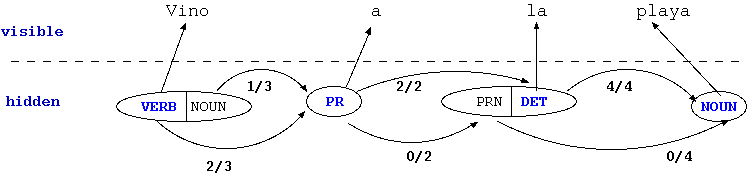
\includegraphics[scale=0.41]{sentence-hmm.png}
  \end{center}
\end{frame}


\section{Tagset definition}

\begin{frame}
  \frametitle{Tagset definition /1}

  To alleviate the problem of data sparseness the sequences of
  morphological tags are grouped into coarse ones

  \begin{exampleblock}{}
    \begin{center}
    \begin{tabular}{ll}
      \textbf{Sequence of tags} & \textbf{Coarse tag}\\
      \hline
      \texttt{noun.m.sg} & NOUN\\
      ... & ...\\
      \texttt{noun.f.pl} & NOUN\\
      \texttt{verb.pres.1p.sg} & VERB.PRESENT \\
      ... & ...\\
      \texttt{verb.pres.3p.pl} & VERB.PRESENT \\
      \texttt{prn.1p.sg} & PRONOUN \\
      \texttt{prn.2p.sg} & PRONOUN \\
      \texttt{prn.3p.sg} & PRONOUN.3P.SG \\
      ... & ...\\
      \texttt{prn.3p.pl} & PRONOUN \\
    \end{tabular}
  \end{center}
  \end{exampleblock}
\end{frame}

\begin{frame}
  \frametitle{Tagset definition /2}

  How to design a tagset:

  \begin{block}{Rules of thumb}
    \begin{itemize}
    \item Group sequences of tags having the same syntactic role under
      the same coarse tag
    \item Do not group under the same coarse tag those sequences of
      tags among which the disambiguator needs to distinguish
    \end{itemize}
  \end{block}

  Starting with a tagset borrowed from a similar language might help
\end{frame}


\begin{frame}
  \frametitle{Tagset definition /3} 

  \begin{exampleblock}{Example of tagset:}
    \begin{footnotesize}
    \begin{alltt}
      <?xml version="1.0" encoding="iso-8859-1"?>\\
      <tagger name="English">\\
      ~<tagset>\\
      ~~...\\
      ~~<def-label name="ADJ">\\
      ~~~<tags-item tags="adj"/>\\
      ~~~<tags-item tags="adj.comp"/>\\
      ~~~<tags-item tags="adj.sup"/> \\
      ~~~<tags-item tags="adj.sint"/>\\
      ~~~<tags-item tags="adj.sint.*"/>\\
      ~~</def-label>\\
      ~~<def-label name="PREP" closed="true">\\
      ~~~<tags-item tags="pr"/>\\
      ~~</def-label>\\
      ~~...\\
      ~</tagset>\\
      ~~...\\
      </tagger>\\
    \end{alltt}
    \end{footnotesize}
  \end{exampleblock}
\end{frame}

\begin{frame}
  \frametitle{Tagset definition /3} 

  \begin{block}{Problems that are very difficult or impossible to solve}
  \begin{itemize}
  \item morphological readings that can appear in the same syntactic contexts\\
    Ex. \texttt{[es]} \emph{cantamos}\\
    ~~$\rightarrow$ \texttt{[en]} \emph{we sing} (\texttt{verb.pri.1p.pl})\\
    ~~$\rightarrow$ \texttt{[en]} \emph{we sang} (\texttt{verb.pii.1p.pl})
  \item homograph where only the lemma changes\\
    Ex. 
    \begin{tabular}{l}
      \texttt{[es]} \emph{creo} (\texttt{verb}): \emph{crear} VS \emph{creer} {\footnotesize (\texttt{[en]} \emph{create} VS \emph{believe})}\\
      %\texttt{[es]} \emph{vendo}: \emph{vendar} VS \emph{vender} {\footnotesize (\texttt{[en]} \emph{bandage} VS \emph{sell})}\\
      \texttt{[ro]} \emph{lunile} (\texttt{noun}): \emph{luni} VS \emph{lună} {\footnotesize (\texttt{[en]} \emph{Mondays} VS \emph{moons})}\\
      \texttt{[sv]} \emph{kullar} (\texttt{noun}): \emph{kull} VS \emph{kulle} {\footnotesize (\texttt{[en]} \emph{crops} VS \emph{hills})}\\
    \end{tabular}
  \item polysemy: recall that part-of-speech ambiguity has nothing to
    do with polysemy
  \end{itemize}
  \end{block}
\end{frame}

\section{Rule-based disambiguation}

\begin{frame}
  \frametitle{Rule-based disambiguation /1}

  \begin{block}{Statistical disambiguator}
    \begin{itemize}
    \item Guarantees that a sentences is completely disambiguated
    \item May make mistakes because it uses a \alert{limited context window}
    \end{itemize}
  \end{block}

  \begin{block}{Constraint grammar rules [optional]}
    \begin{itemize}
    \item Do not guarantee that a sentences is always completely
      disambiguated
      \begin{itemize}
      \item They must be applied before the statistical
        disambiguator
      \end{itemize}
    \item Can reduced (or even solve) the ambiguity
    \item Can use a \alert{variable-length context window}
    \end{itemize}
  \end{block}
\end{frame}

\begin{frame}
  \frametitle{Rule-based disambiguation /2}

  \begin{exampleblock}{Example of constraint grammar rule:}
    \begin{small}
    \begin{alltt}
       LIST DET-DEM = (det dem);\\
       LIST PRON-DEM = (prn dem);\\

       REMOVE PRON-DEM IF (0 PRON-DEM) (0 DET-DEM) (1C N);
    \end{alltt}
    \end{small}
  \end{exampleblock}

  \begin{block}{}
    Remove a reading of demonstrative pronoun IF
    \begin{itemize}
    \item The current word can be a demonstrative pronoun, AND
    \item The current word can also be a demonstrative determiner, AND
    \item The first word to the right can ONLY be a noun
    \end{itemize}
  \end{block}
\end{frame}

\begin{frame}
  \frametitle{Rule-based disambiguation /3}

  \begin{exampleblock}{Another example of constraint grammar rule:}
    \begin{small}
    \begin{alltt}
      LIST PAST = (pii);\\
      LIST PRES = (pri);\\
      LIST TEMP-ADV-PAST = ("ayer" adv) ("antes" adv);\\

      SELECT PAST IF (0 PAST) (0 PRES) (-1 TEMP-ADV-PAST);
    \end{alltt}
    \end{small}
  \end{exampleblock}

  \begin{block}{}
    Select past tense IF
    \begin{itemize}
    \item The current word can be a verb in past tense, AND
    \item The current word can also be a verb in present tense, AND
    \item The first word to the left is an adverb that indicates past
    \end{itemize}
  \end{block}
\end{frame}


\begin{frame}
  \frametitle{Some commands}

  \begin{block}{Running the tagger}
    \texttt{\$ echo} ``This is an example'' \texttt{|}\\
    \texttt{ lt-proc -a en-es.automorf.bin |}\\
    \texttt{ apertium-tagger -g en-es.prob}
  \end{block}

  \begin{block}{Seeing how sequences of tags are mapped into coarse ones}
    \texttt{\$ echo} ``This is an example'' \texttt{|}\\
    \texttt{ lt-proc -a en-es.automorf.bin |}\\
    \texttt{ apertium-tagger-readwords -p en-es.prob} 
    
    OR
    
    \texttt{\$ echo} ``This is an example'' \texttt{|}\\
    \texttt{ lt-proc -a en-es.automorf.bin |}\\
    \texttt{ apertium-tagger-readwords -x } \\
    \texttt{ apertium-en-es.en.tsx}
  \end{block}
\end{frame}

\end{document}
